% ============================================================================
% jfr2026.tex
% JFR 2026 — Évaluation objective de la qualité d'image en radiologie
% interventionnelle : quelles métriques ?
%
% Compilation : ./build.sh (latexmk : lualatex + biber, sortie dans build/)
% Plan détaillé, texte d'oral et minutage : plan_JFR2026.md
% Modèle : commun/preambule-presentation.tex (copié du projet cours), palette JFR.
% Règles de rédaction : CLAUDE.md (une idée par diapo, pas de sous-titre,
% sources en bas via \src, un \highlight par diapo).
% ============================================================================

\documentclass[aspectratio=169, 11pt]{beamer}
\newcommand{\commun}{commun}
\newcommand{\palettecourante}{JFR}
\input{\commun/preambule-presentation}
\usepackage{jfr2026}      % \src{cles} en bas de diapo, \refslide{cles}, pages titre/fin
\graphicspath{{../figures/}}
% \setbeameroption{show notes on second screen=right}   % notes d'orateur

\title[Qualité d'image en radiologie interventionnelle : quelles métriques ?]
  {Évaluation objective de la qualité d'image en radiologie interventionnelle : quelles métriques ?}
\subtitle{Du bruit au mouvement : mettre le temps dans la qualité image}
\author[L. Ammour, H. Desal]{Dr Luis Ammour, Pr Hubert Desal}
\institute[CHU Nantes]{CHU de Nantes}
\date[JFR 2026]{\footnotesize\makebox[0pt][l]{Journées Francophones de Radiologie Diagnostique et Interventionnelle}\\ 8 octobre 2026}

\begin{document}

% --------------------------- DIAPO 1 · TITRE (0:00 → 0:20) ------------------
\pagetitre
\note{Merci. Je vais vous parler de ce que nous mesurons aujourd'hui pour qualifier une image d'interventionnel, de ce que ces mesures ne voient pas, et de ce que nous devrions mesurer. J'irai vite sur la physique et je vous montrerai des images acquises à Nantes.}

% ============================================================================
\section{État des lieux}

% --------------------------- DIAPO 2 (0:20 → 1:30) --------------------------
\begin{frame}{Pourquoi l'interventionnel est un cas à part}
  \begin{itemize}
    \item \textbf{La dose compte :} le seuil des effets déterministes peut être atteint sur les procédures longues.
    \item \textbf{L'image est un flux :} 7,5 à 30 images/s, cathéter en mouvement. La tâche clinique porte sur la \emph{séquence}, pas sur l'image isolée.
    \item \textbf{Le traitement constructeur fait l'image :} filtres temporels et rehaussement non linéaire, opaques, pilotés par la dose.
  \end{itemize}
  \vspace{0.2cm}
  {\color{Sage}\bfseries Anthony et al. 2022\srcref{anthony2022} :} deux salles comparables en débit de kerma et en résolution limite, deux traitements opposés, lissage spatial et \highlight{efficacité SNR $\times$ 4} d'un côté, rehaussement de contours et \highlight{MTF à 50\,\% $\times$ 1,5} de l'autre.
  \src{anthony2022}
  \note{Trois choses distinguent l'interventionnel. D'abord la dose : sur des procédures longues, on atteint le seuil des effets déterministes, la qualité d'image n'est donc pas un luxe, c'est la contrepartie d'une dose qu'on ne peut pas augmenter. Ensuite l'image est un flux : ce que le radiologue regarde, c'est une séquence à 7,5 ou 15 images par seconde, avec un cathéter qui bouge ; l'image isolée n'est pas l'objet clinique. Enfin, depuis plus de dix ans, c'est le traitement constructeur qui fait l'image. Anthony et ses collègues ont comparé deux salles qui délivrent un débit de dose comparable : Siemens combine un filtre temporel léger et un lissage spatial agressif, Philips un filtre temporel un peu plus marqué et un rehaussement de contours. Les images sont visiblement différentes. Leur résolution limite et leur résolution spatio-temporelle sont pourtant comparables, et les auteurs le disent eux-mêmes : leurs métriques d'efficacité de dose, calculées sur images traitées, ne caractérisent pas complètement ces systèmes. C'est tout le problème.}
\end{frame}

% --------------------------- DIAPO 3 (1:30 → 3:00) --------------------------
\begin{frame}{Ce que nous mesurons aujourd'hui}
  \small
  \renewcommand{\arraystretch}{1.0}
  \begin{tabular}{@{}>{\raggedright\arraybackslash}p{1.6cm}>{\raggedright\arraybackslash}p{3.7cm}>{\raggedright\arraybackslash}p{3.8cm}>{\raggedright\arraybackslash}p{3.5cm}@{}}
    & {\color{Slate}\bfseries Constructeur} & {\color{Slate}\bfseries Recette et CQ} & {\color{Slate}\bfseries Clinique} \\
    \midrule
    {\color{Sage}\bfseries Source} & DQE selon IEC 62220-1-3\srcref{iec2008}, via MTF et NPS & ANSM 2016\srcref{ansm2016}, TG-272\srcref{lin2022}, EFOMP 2024\srcref{efomp2024} & Cotation visuelle\srcref{bath2007}, études de lecture \\
    \noalign{\vskip 1.5pt{\color{StoneLight}\hrule height 0.5\lightrulewidth}\vskip 1.5pt}
    {\color{Sage}\bfseries Contenu} & Images brutes, faisceau RQA5 sans grille ; une DQE par trame & Résolution, bas contraste, uniformité ; CHO 2D par trame ; roue tournante & Images traitées, flux réel ; qualité perçue ou détection \\
    \noalign{\vskip 1.5pt{\color{StoneLight}\hrule height 0.5\lightrulewidth}\vskip 1.5pt}
    {\color{Sage}\bfseries Limites} & Avant traitement, sans patient ; lag retiré, filtre invisible & Roue lue à l'œil, \textbf{qualitatif} ; MTF et NPS sans traitement, pas de DQE & Subjectif, coûteux, tardif \\
  \end{tabular}
  \vspace{0.05cm}
  \begin{center}
    \highlight{statique} \quad \highlight{avant traitement} \quad \highlight{ou subjectif}
  \end{center}
  \vspace{-0.2cm}
  \src{iec2008,ansm2016,lin2022,efomp2024,bath2007}
  \note{Voilà ce que nous avons dans la boîte à outils. Côté constructeur, la DQE selon la norme IEC : c'est une excellente métrique, mais elle est mesurée sur des images brutes, offset, gain et pixels défectueux corrigés, rien d'autre, avec un faisceau RQA en laboratoire, sans grille ni diffusé. Et dans le cas dynamique c'est une DQE par frame, où le lag est mesuré pour être retiré de la NPS, pas pour être rapporté. Côté recette, le rapport TG-272 de l'AAPM et le protocole EFOMP de 2024 : résolution, bas contraste sur objets-tests, uniformité, et pour le mouvement une roue tournante lue à l'œil ; le rapport écrit lui-même qu'il est « prématuré » de proposer un test pour les systèmes optimisés en CNR, faute de méthode et de fantôme (§ 2.3.5). L'EFOMP a fait un pas important en introduisant des observateurs mathématiques, appliqués frame par frame, et un facteur de lag dans son SNR² par seconde. Mais le seul objet réellement mobile normalisé reste la roue à rayons NEMA, dont la lecture est qualitative. Côté clinique enfin, le visual grading et les études de lecteurs : c'est ce qui compte vraiment, mais c'est coûteux, peu reproductible, et cela arrive après l'achat. Retenez la ligne du bas : tout ce que nous mesurons est soit statique, soit mesuré avant le traitement, soit subjectif. Si le temps presse : 60 s en sautant la colonne clinique.}
\end{frame}

% --------------------------- DIAPO 4 (3:00 → 4:00) --------------------------
\begin{frame}{Trois angles morts}
  \centering
  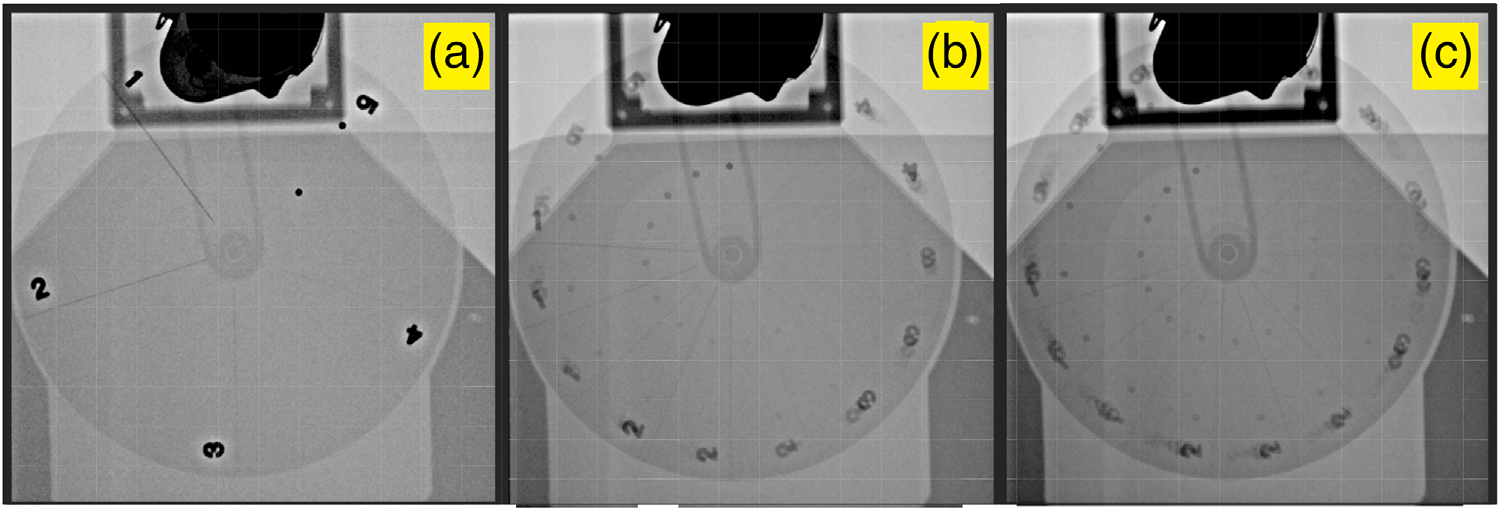
\includegraphics[width=0.66\linewidth]{nema_roue_lag.png}
  \sourceimage{Roue NEMA XR-21 à 7,5 i/s : sans lag, lag modéré, lag extrême. TG-272, fig. 17.}
  \vspace{0.1cm}
  \raggedright
  \begin{itemize}
    \item \textbf{Lag} : rémanence du détecteur, le bruit d'une trame est corrélé à la précédente\srcref{konst2021}.
    \item \textbf{Filtre récursif} : l'image affichée mélange la trame courante et la précédente. Moins de bruit, plus de flou, réglage rarement documenté\srcref{konst2021}.
    \item \textbf{Non-linéarité} : la réponse dépend du contraste et de la dose, il n'y a plus \emph{une} MTF\srcref{monnin2021}.
  \end{itemize}
  \src{konst2021,monnin2021}
  \note{Trois phénomènes échappent aux mesures statiques. La rémanence, celle du détecteur, qui garde une trace des frames précédentes, ou celle du traitement : ce que vous voyez ici sur la roue NEMA qui se dédouble quand l'intégration temporelle augmente. Le filtre récursif : l'image affichée est un mélange pondéré de la frame courante et de l'image précédente ; on gagne beaucoup en bruit, on perd en netteté du mouvement, et le coefficient de mélange est rarement documenté, jamais sous une forme comparable d'une marque à l'autre (K-factor Siemens, TNRT Philips, propriétaire GE ; sur un Artis Q, Villa 2026 doit estimer les modes automatiques par trois méthodes). Et la non-linéarité des traitements récents : leur réponse dépend du contraste et de la dose, il n'y a plus une MTF. Le point commun : ces trois effets sont temporels ou non linéaires. Une DQE statique sur image brute est aveugle aux trois.}
\end{frame}

% ============================================================================
\section{Mesurer le filtre récursif}

% --------------------------- DIAPO 5 (4:00 → 5:40) --------------------------
\begin{frame}{Trois images pour mesurer le filtre}
  \begin{columns}[T]
    \begin{column}{0.62\textwidth}
      \textbf{Filtre récursif}
      \vspace{-0.25cm}
      {\[ I[n] = \tfrac{1}{K}\bigl( S[n] + (K-1)\,I[n-1] \bigr) \]}
      \par\vspace{-0.2cm}
      {\tiny\color{StoneLight} $I$ : image affichée, $S$ : trame acquise, $n$ : numéro de trame, $K$ : K-factor de la console.\par}
      \vspace{0.12cm}

      \textbf{Méthode de {\color{Sage}Konst et al. 2021}\srcref{konst2021}}
      \begin{enumerate}
        \item Fantôme de PMMA, protocole clinique.
        \item Deux trames voisines $B$, $C$ ; une trame éloignée $A$.
        \item {\small $\displaystyle K = \frac{R+1}{2R}, \qquad R = \frac{\mathrm{Var}(C-B)}{\mathrm{Var}(B+C) - 4\sigma_{\mathrm{fixe}}^2}$}\\[4pt]
          {\small $\sigma_{\mathrm{fixe}}^2$ : bruit de structure fixe, $\sigma_{\mathrm{fixe}}^2 = \mathrm{Cov}(A, C) = \tfrac{1}{4}\bigl[\mathrm{Var}(A+C) - \mathrm{Var}(C-A)\bigr]$.}\\
          {\tiny\color{StoneLight} Var : variance des pixels dans la ROI.}
      \end{enumerate}
    \end{column}
    \begin{column}{0.33\textwidth}
      \centering
      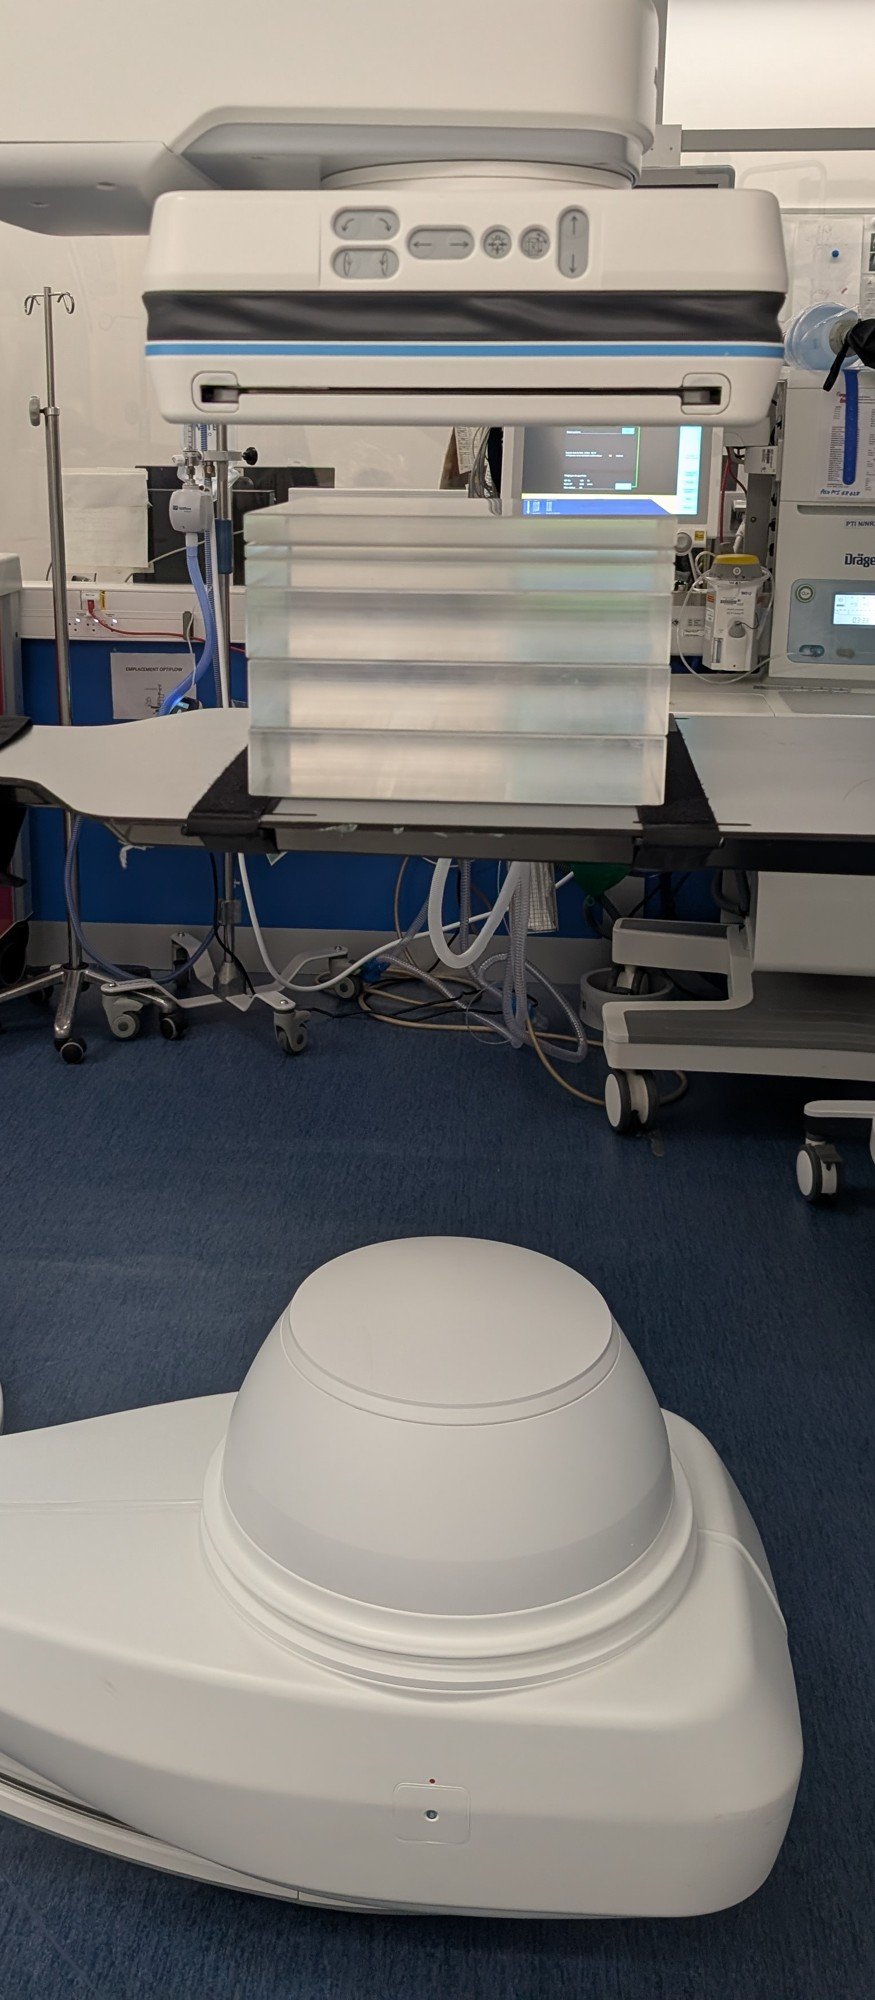
\includegraphics[height=6.2cm]{montage_icono.jpg}
      \sourceimage{PMMA 20 cm entre tube et détecteur, Siemens Artis Icono biplan, CHU Nantes.}
    \end{column}
  \end{columns}
  \src{konst2021}
  \note{On peut mesurer ce filtre. Konst et ses collègues ont montré en 2021 qu'il suffit de trois images d'un fantôme uniforme : deux frames consécutives, une frame éloignée. Le filtre corrèle le bruit des frames voisines ; l'image différence annule ce bruit corrélé, l'image somme l'amplifie ; le ratio des deux variances donne directement le coefficient du filtre, la frame éloignée servant à retirer le bruit de structure fixe du détecteur. Exactitude de l'ordre du pour cent, sur quatre arceaux mobiles (GE, Philips, Siemens et Ziehm), avec des coefficients qui vont de « pas de filtre » à une moyenne effective sur treize images, et qui, chez certains constructeurs, changent avec la dose. Voici ce que nous avons mesuré à Nantes [décrire : sur telle salle, β passe de … en scopie haute dose à … en basse dose, soit un moyennage sur … à … frames]. [Si confirmé :] Autrement dit, quand on baisse la dose, ce système ne baisse pas la qualité apparente : il moyenne davantage dans le temps, et la traînée derrière un cathéter s'allonge. [Sinon : Anthony 2022 montre qu'un constructeur peut au contraire garder un filtre temporel léger et lisser dans l'espace.] Dans les deux cas, c'est invisible dans une DQE, trompeur dans un TO.10, et absent du rapport de recette. Trois images suffisent à le rendre visible. Si un physicien demande « et les modes automatiques ? » : Villa 2026, Artis Q, le K mesuré sur fond uniforme dépasse le K déduit d'un objet mobile, le filtre se désactive localement autour du mouvement ; d'où le mot « minorant ».}
\end{frame}

% --------------------------- DIAPO 5 bis : résultats CHU Nantes ---------------
\begin{frame}{Mesuré à Nantes sur l'Artis Icono}
  \centering
  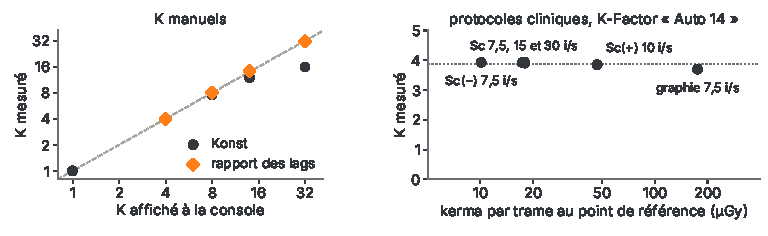
\includegraphics[width=0.90\linewidth]{beta_icono.pdf}
  \sourceimage{Siemens Artis Icono biplan, PMMA 20 cm, 24 boucles, deux répétitions par protocole.}
  \raggedright
  \small
  \begin{itemize}
    \item \textbf{Rapport des lags} (non publié) : même principe que Konst\srcref{konst2021} avec une trame de plus pour éliminer le bruit non filtré.
    \item \textbf{$K$ manuels} : retrouvés de 1 à 32, répétabilité 0,4\,\%.
    \item \textbf{Protocoles cliniques} : \highlight{$K = 3{,}9$} partout, le filtrage ne dépend pas de la dose.
  \end{itemize}
  \src{konst2021}
\end{frame}

% --------------------------- DIAPO 6 (5:40 → 6:40) --------------------------
\begin{frame}{Le paradoxe du disque statique}
  \begin{columns}[T]
    \begin{column}{0.47\textwidth}
      \centering
      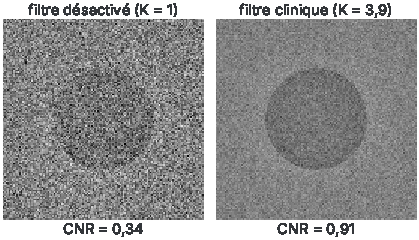
\includegraphics[width=\linewidth]{disque_icono.pdf}
      \sourceimage{Disque Cu 0,1 mm sur PMMA 20 cm, Sc(−) 7,5 i/s, même dose, même fenêtre. Artis Icono, CHU Nantes.}
      \vspace{0.05cm}
      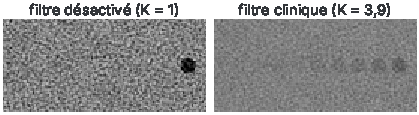
\includegraphics[width=\linewidth]{mobile_icono.pdf}
      \sourceimage{Simulation : bille de 3 mm à 30 mm/s ajoutée aux trames réelles sans filtre, filtre récursif appliqué numériquement.}
    \end{column}
    \begin{column}{0.49\textwidth}
      \small
      \begin{itemize}
        \item \textbf{Objet immobile}, même dose : CNR de 0,34 à 0,91, soit $\times\,2{,}6$ ($\sqrt{2K-1}$\srcref{konst2021}).
      \end{itemize}
      \vspace{0.05cm}
      Plus on filtre, meilleur est le CNR statique : la métrique récompense \highlight{ce qui dégrade le mouvement}.

      \vspace{0.3cm}
      {\color{Sage}\bfseries Villa et al. 2026\srcref{villa2026} :} un mode adaptatif filtre moins autour de l'objet, la traînée réelle peut être réduite.
    \end{column}
  \end{columns}
  \src{konst2021,villa2026}
  \note{Voici le piège. Un disque de cuivre immobile, le même que celui de Monnin, en scopie basse et haute dose. Le CNR mesuré sur la frame affichée est [meilleur / à peine dégradé] en basse dose : le filtre a compensé. Une recette sur objet statique conclurait que tout va bien. Mais regardez la même série dans le temps : la part d'information réellement nouvelle à chaque frame [la bande passante temporelle / l'image différence] s'est effondrée. Le CNR statique récompense exactement ce qui abîme la visibilité d'un guide en mouvement. C'est pour cela qu'il nous faut des métriques qui portent la dimension temporelle. Rappel physique : en régime établi le CNR de la frame affichée monte d'un facteur racine de (2−β)/β, soit ×4,9 pour β = 0,08.}
\end{frame}

% ============================================================================
\section{Mettre le temps dans la DQE}

% --------------------------- DIAPO 7 (6:40 → 7:50) --------------------------
\begin{frame}{La DQE spatio-temporelle}
  % pas d'accolade en tête de corps : beamer la lirait comme un sous-titre de frame
  \textcolor{Sage}{\bfseries Friedman et Cunningham 2010\srcref{friedman2010} :}
  \vspace{-0.1cm}
  \begin{columns}[T]
    \begin{column}{0.5\textwidth}
      \eqbox{\mathrm{DQE}(u, v, \nu) = \frac{\mathrm{MTF}^2(u, v, \nu)}{\dot{q}\cdot\mathrm{NNPS}(u, v, \nu)}}
      \par\vspace{-0.15cm}
      {\tiny\color{StoneLight} $u$, $v$ : fréquences spatiales ; $\nu$ : fréquence temporelle\srcref{friedman2008} ; $\dot{q}$ : débit de fluence incident ; $\mathrm{NNPS} = \mathrm{NPS}/\bar{d}^{\,2}$\srcref{siewerdsen2002}.\par}
      \vspace{0.3cm}

      Mesurée sans traitement à 30 i/s, elle chute d'environ \highlight{50\,\% à 15 Hz} par repliement temporel du bruit.
      \vspace{0.2cm}

      Elle voit le lag et le repliement, elle est \textbf{aveugle au filtre temporel}.
    \end{column}
    \begin{column}{0.46\textwidth}
      \centering
      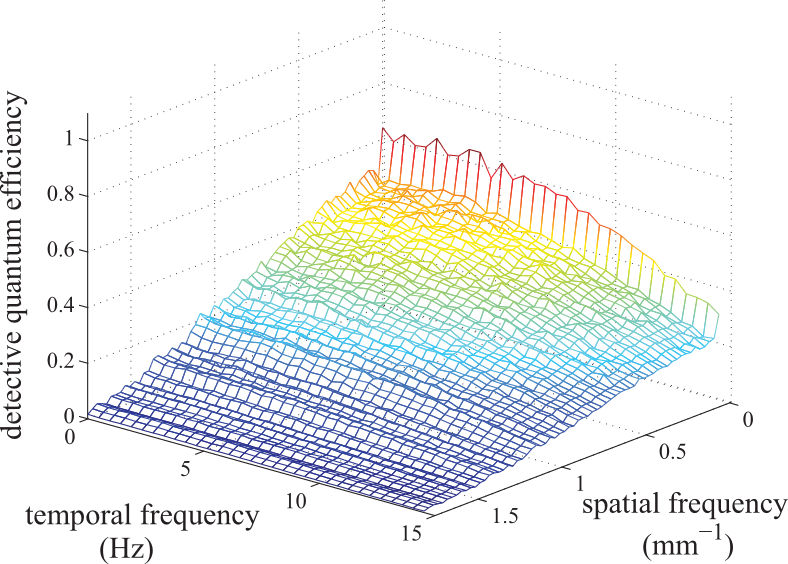
\includegraphics[width=\linewidth]{dqe_friedman_t.png}
      \sourceimage{Friedman et Cunningham 2010, fig. 6.}
    \end{column}
  \end{columns}
  \src{friedman2010,friedman2008,siewerdsen2002}
  \note{Le cadre théorique existe depuis plus de quinze ans. Cunningham, puis Friedman et Cunningham, ont écrit la DQE avec une troisième dimension, la fréquence temporelle. À fréquence temporelle nulle, c'est en première approximation la DQE que tout le monde connaît ; quand la fréquence temporelle monte, la DQE chute, d'environ 50 \% à 15 hertz sur leur banc, un amplificateur de brillance en scopie continue, sans traitement. Cette chute, c'est le repliement temporel du bruit : une dégradation qu'aucune mesure statique ne voyait. Mais Friedman le dit lui-même : un filtre temporel linéaire atténue le signal et le bruit de la même façon, et ne change pas cette DQE. Elle voit le lag et le repliement ; elle est aveugle au filtre. Et elle a deux autres limites, instructives. Elle suppose un système linéaire, donc elle a été mesurée sans traitement constructeur. Et une DQE tridimensionnelle décrit la chaîne, pas ce qu'on voit dans une frame. MTF temporelle par bord incliné mobile (Friedman 2008), NPS 3D par FFT d'une pile de frames (Siewerdsen 2002).}
\end{frame}

% --------------------------- DIAPO 8 (7:50 → 9:00) --------------------------
\begin{frame}{La DQE de la chaîne complète, traitement compris}
  \twocols{%
    \centering
    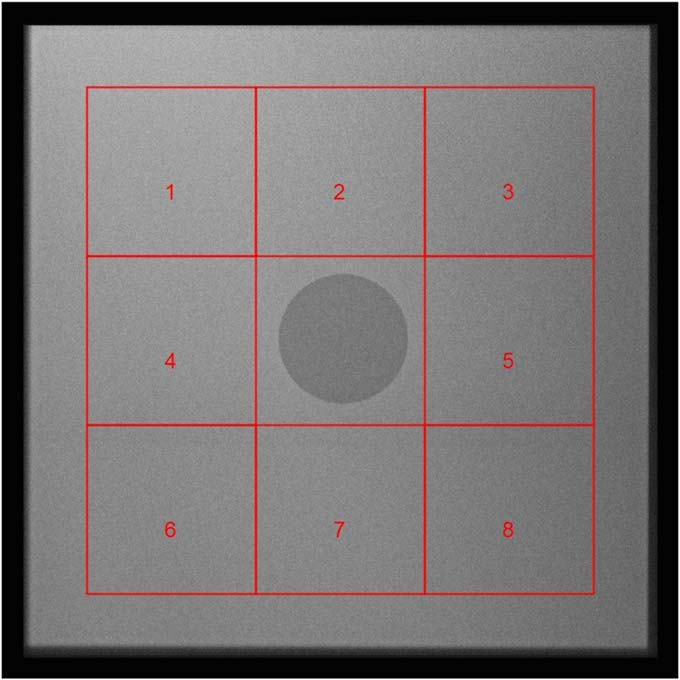
\includegraphics[height=2.6cm]{disque_monnin.png}
    \sourceimage{Disque Cu 0,1 mm en translation. Monnin et al. 2021.}
    \vspace{0.05cm}
    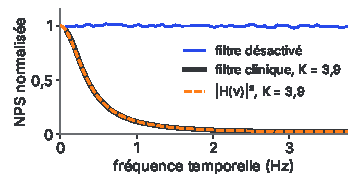
\includegraphics[width=0.95\linewidth]{nps_icono.pdf}
    \sourceimage{NPS temporelle mesurée à Nantes, Artis Icono, Sc 7,5 i/s.}
  }{%
    \small
    \textcolor{Sage}{\bfseries Monnin et al. 2021\srcref{monnin2021} :}
    \vspace{0.1cm}

    \textbf{Faible contraste, traitement activé.} Pour un disque de 0,1 mm Cu, le traitement se comporte à peu près linéairement : mesure avec grille, diffusé et traitement en place.
    \vspace{0.25cm}

    \textbf{DQE de trame} : signal intégré avec la MTF temporelle, bruit avec la NPS temporelle, sur la chaîne complète.
    \vspace{0.25cm}

    \textbf{La DQE de trame est} \highlight{invariante au filtre temporel} : le compromis bruit / mouvement se lit à part, dans la \textbf{MTF temporelle}.
  }
  \src{monnin2021}
  \note{Monnin et ses collègues, à Lausanne, ont répondu aux deux limites. Pour la linéarité : un disque de cuivre de faible contraste, pour lequel le traitement constructeur se comporte approximativement comme un système linéaire ; on peut donc mesurer traitement activé, grille et fantôme diffusant en place. Pour le lien avec la frame : ils intègrent séparément le signal et le bruit sur la bande temporelle et obtiennent une DQE de frame : 0,65 pour deux systèmes Siemens (Cios Fusion, Artis Zee) à vingt centimètres d'eau, moins sur les faibles épaisseurs à cause de la grille. Et voici le point intéressant : cette DQE ne bouge pratiquement pas quand on change le filtre temporel, parce que le filtre atténue le signal et le bruit de la même façon. Ce qui bouge, c'est la MTF temporelle. Autrement dit, même une DQE spatio-temporelle ne dit pas à elle seule ce que fait le filtre ; il faut lire les deux. C'est, à ma connaissance, la seule DQE de la chaîne complète, post-traitement compris. Elle n'est ni dans TG-272 ni dans l'EFOMP. C'est la mesure que nous n'avons pas encore à Nantes, faute de fantôme mobile fiable. Attention : la formule de la diapo 25 du webinaire est le NEQ de frame (éq. 22), pas la DQE de frame (éq. 23).}
\end{frame}

% --------------------------- DIAPO 9 (9:00 → 10:00) -------------------------
\begin{frame}{De la DQE à la tâche}
  \small
  \begin{columns}[T]
    \begin{column}{0.31\textwidth}
      \textbf{Le principe}\\[2pt]
      La qualité d'image, c'est la performance à une tâche : voir un guide qui bouge, pas un disque immobile. Du NEQ de trame, un observateur mathématique tire une détectabilité $d'$.
    \end{column}
    \begin{column}{0.31\textwidth}
      \textbf{Pourquoi c'est nécessaire}\\[2pt]
      Le seuil visuel sur objet-test ne voit que de grands changements, 8 à 20\,\% d'écart par observateur\srcref{tapiovaara2004}. Le scanner a basculé avec le TG-233\srcref{samei2019} : TTF et $d'$ remplacent MTF et CNR.
    \end{column}
    \begin{column}{0.31\textwidth}
      \textbf{C'est faisable en RI}\\[2pt]
      Observateurs spatio-temporels sur cibles mobiles, à 12\,\% des lecteurs humains\srcref{ingraito2023}. Un $d'$ spatio-temporel sur la chaîne complète : Monnin et al. (non publié, présenté aux JS SFPM 2023)\srcref{viry2023}.
    \end{column}
  \end{columns}
  \vspace{0.25cm}
  \centering
  Il manque \highlight{une tâche clinique} définie avec les radiologues.
  \src{tapiovaara2004,samei2019,ingraito2023,viry2023}
  \note{Dernière marche : la tâche. L'ICRU le dit depuis 1996, la qualité d'image n'a de sens que par rapport à une tâche : voir un guide de 0,014 pouce qui bouge, pas un disque immobile. Les observateurs mathématiques permettent de calculer un indice de détectabilité, reproductible, là où la lecture visuelle d'un objet-test, Tapiovaara l'a montré, ne l'est pas. Le scanner a fait ce basculement il y a quelques années avec le TG-233, précisément parce que la reconstruction itérative avait cassé le cadre linéaire. En interventionnel, tout existe : des observateurs spatio-temporels sur cibles mobiles à Monza, des observateurs de Hotelling sur fonds anthropomorphes avec objets mobiles à la Mayo, et l'EFOMP a déjà mis un observateur mathématique, frame par frame, dans son protocole 2024. Il manque la cible mobile et le lien avec une tâche clinique définie par vous, les radiologues. Dire « détectabilité » plutôt que d′ ; ne prononcer « Hotelling » qu'une fois. Si le temps presse : 40 s, garder seulement la colonne de droite.}
\end{frame}

% ============================================================================
\section{Et maintenant}

% --------------------------- DIAPO 10 (10:00 → 11:00) -----------------------
\begin{frame}{L'IA rend ce basculement urgent}
  \twocols{%
    \textbf{Ce qui arrive en salle}
    \begin{itemize}
      \item Débruiteur par apprentissage chez Siemens\srcref{madoff2026}, nouvelle chaîne spatio-temporelle chez Philips\srcref{assar2026}.
      \item Une DSA générative : kerma $-$67\,\% dans un essai randomisé de 1068 patients\srcref{zhao2026}.
      \item Évaluées par des lecteurs, sans métrique physique de la chaîne.
    \end{itemize}
  }{%
    \textbf{Ce que l'on sait des métriques}
    \begin{itemize}
      \item La MTF d'une reconstruction par apprentissage dépend du contraste\srcref{solomon2020}.
      \item Un observateur calculé en Fourier \emph{surestime} le bénéfice du débruitage\srcref{poludniowski2026}.
      \item Son bruit n'est plus stationnaire : plus fort près des bords, plus faible dans les zones uniformes\srcref{solomon2020}.
    \end{itemize}
  }
  \src{madoff2026,assar2026,zhao2026,solomon2020,poludniowski2026}
  \note{Et pourquoi maintenant. Les débruiteurs par apprentissage profond arrivent en salle : Optiq AI chez Siemens (préprint, non relu par les pairs), SmartIQ chez Philips, et une angiographie soustraite générative qui divise la dose par trois dans un essai randomisé publié dans Nature Medicine. Toutes ces études sont cliniques, avec des lecteurs ; aucune ne publie de métrique physique de la chaîne. Or on sait du scanner que ces algorithmes ont une MTF qui dépend du contraste et de la dose, et qu'un observateur calculé en Fourier surestime le bénéfice du débruitage. Un algorithme qui a appris à quoi ressemble un guide peut en dessiner un. La protection la plus directe est une tâche, mesurée sur la chaîne complète, avec des cibles qui bougent. Prudence : dire « une DSA générative », « réduction de dose des deux tiers dans un essai randomisé », ne pas dire « synthétique ».}
\end{frame}

% --------------------------- DIAPO 11 (11:00 → 12:00) -----------------------
\begin{frame}{Ce que nous pouvons faire dès demain}
  \begin{enumerate}
    \item \textbf{À la recette et au suivi} : mesurer $K$ sur chaque protocole. Un fantôme de PMMA, trois images, quelques minutes. L'écrire dans le rapport, à côté de la dose.
    \item \textbf{Dans les protocoles nationaux} : porter la NPS temporelle, la MTF temporelle et le NEQ de trame ; viser la DQE de trame pour la normalisation.
    \item \textbf{En recherche clinique} : définir des tâches de référence et un observateur commun ; étudier les nouveaux algorithmes d'IA.
  \end{enumerate}
  \vspace{0.4cm}
  \centering
  \highlight{Une DQE ne dit pas ce que vous voyez.}
  \note{Trois leviers. Dès demain : mesurer le coefficient du filtre temporel à la recette, trois images, quelques minutes par protocole, et l'écrire dans le rapport à côté de la dose. Ensuite : porter la NPS temporelle, la MTF temporelle et le NEQ de frame dans les protocoles (le NEQ ne demande pas la mesure du diffusé, la DQE de frame si). Enfin, avec vous : définir deux ou trois tâches cliniques de référence et un observateur commun, et les exiger pour tout algorithme d'IA. Une DQE ne dit pas ce que vous voyez. Mesurez le temps, mesurez la chaîne complète, mesurez la tâche. Merci.}
\end{frame}

% ============================================================================
\appendix

% --------------------------- RÉFÉRENCES (non commentées) --------------------
\refslide{anthony2022,konst2021,viry2023,iec2008,ansm2016,lin2022,efomp2024,friedman2010,monnin2021,ingraito2023,poludniowski2026,zhao2026}

% --------------------------- PAGE DE FIN -------------------------------------
\pagefin[fin_bruit_qr.png]{}

\end{document}
